\documentclass[12pt,a4paper]{article}

%\usepackage[left=1.5cm,right=1.5cm,top=1cm,bottom=2cm]{geometry}
\usepackage[in, plain]{fullpage}
\usepackage{array}
\usepackage{../../../pas-math}
\usepackage{../../../moncours}


%\usepackage{pas-cours}
%-------------------------------------------------------------------------------
%          -Packages nécessaires pour écrire en Français et en UTF8-
%-------------------------------------------------------------------------------
\usepackage[utf8]{inputenc}
\usepackage[frenchb]{babel}
\usepackage[T1]{fontenc}
\usepackage{lmodern}
\usepackage{textcomp}



%-------------------------------------------------------------------------------

%-------------------------------------------------------------------------------
%                          -Outils de mise en forme-
%-------------------------------------------------------------------------------
\usepackage{hyperref}
\hypersetup{pdfstartview=XYZ}
%\usepackage{enumerate}
\usepackage{graphicx}
\usepackage{multicol}
\usepackage{tabularx}
\usepackage{multirow}


\usepackage{anysize} %%pour pouvoir mettre les marges qu'on veut
%\marginsize{2.5cm}{2.5cm}{2.5cm}{2.5cm}

\usepackage{indentfirst} %%pour que les premier paragraphes soient aussi indentés
\usepackage{verbatim}
\usepackage{enumitem}
\usepackage[usenames,dvipsnames,svgnames,table]{xcolor}

\usepackage{variations}

%-------------------------------------------------------------------------------


%-------------------------------------------------------------------------------
%                  -Nécessaires pour écrire des mathématiques-
%-------------------------------------------------------------------------------
\usepackage{amsfonts}
\usepackage{amssymb}
\usepackage{amsmath}
\usepackage{amsthm}
\usepackage{tikz}
\usepackage{xlop}
%-------------------------------------------------------------------------------



%-------------------------------------------------------------------------------


%-------------------------------------------------------------------------------
%                    - Mise en forme avancée
%-------------------------------------------------------------------------------

\usepackage{ifthen}
\usepackage{ifmtarg}


\newcommand{\ifTrue}[2]{\ifthenelse{\equal{#1}{true}}{#2}{$\qquad \qquad$}}

%-------------------------------------------------------------------------------

%-------------------------------------------------------------------------------
%                     -Mise en forme d'exercices-
%-------------------------------------------------------------------------------
%\newtheoremstyle{exostyle}
%{\topsep}% espace avant
%{\topsep}% espace apres
%{}% Police utilisee par le style de thm
%{}% Indentation (vide = aucune, \parindent = indentation paragraphe)
%{\bfseries}% Police du titre de thm
%{.}% Signe de ponctuation apres le titre du thm
%{ }% Espace apres le titre du thm (\newline = linebreak)
%{\thmname{#1}\thmnumber{ #2}\thmnote{. \normalfont{\textit{#3}}}}% composants du titre du thm : \thmname = nom du thm, \thmnumber = numéro du thm, \thmnote = sous-titre du thm

%\theoremstyle{exostyle}
%\newtheorem{exercice}{Exercice}
%
%\newenvironment{questions}{
%\begin{enumerate}[\hspace{12pt}\bfseries\itshape a.]}{\end{enumerate}
%} %mettre un 1 à la place du a si on veut des numéros au lieu de lettres pour les questions 
%-------------------------------------------------------------------------------

%-------------------------------------------------------------------------------
%                    - Mise en forme de tableaux -
%-------------------------------------------------------------------------------

\renewcommand{\arraystretch}{1.7}

\setlength{\tabcolsep}{1.2cm}

%-------------------------------------------------------------------------------



%-------------------------------------------------------------------------------
%                    - Racourcis d'écriture -
%-------------------------------------------------------------------------------

% Angles orientés (couples de vecteurs)
\newcommand{\aopp}[2]{(\vec{#1}, \vec{#2})} %Les deuc vecteurs sont positifs
\newcommand{\aopn}[2]{(\vec{#1}, -\vec{#2})} %Le second vecteur est négatif
\newcommand{\aonp}[2]{(-\vec{#1}, \vec{#2})} %Le premier vecteur est négatif
\newcommand{\aonn}[2]{(-\vec{#1}, -\vec{#2})} %Les deux vecteurs sont négatifs

%Ensembles mathématiques
\newcommand{\naturels}{\mathbb{N}} %Nombres naturels
\newcommand{\relatifs}{\mathbb{Z}} %Nombres relatifs
\newcommand{\rationnels}{\mathbb{Q}} %Nombres rationnels
\newcommand{\reels}{\mathbb{R}} %Nombres réels
\newcommand{\complexes}{\mathbb{C}} %Nombres complexes


%Intégration des parenthèses aux cosinus
\newcommand{\cosP}[1]{\cos\left(#1\right)}
\newcommand{\sinP}[1]{\sin\left(#1\right)}


%Probas stats
\newcommand{\stat}{statistique}
\newcommand{\stats}{statistiques}
%-------------------------------------------------------------------------------

%-------------------------------------------------------------------------------
%                    - Mise en page -
%-------------------------------------------------------------------------------

\newcommand{\twoCol}[1]{\begin{multicols}{2}#1\end{multicols}}


\setenumerate[1]{font=\bfseries,label=\textit{\alph*})}
\setenumerate[2]{font=\bfseries,label=\arabic*)}


%-------------------------------------------------------------------------------
%                    - Elements cours -
%-------------------------------------------------------------------------------





%\makeatletter
%\renewcommand*{\@seccntformat}[1]{\csname the#1\endcsname\hspace{0.1cm}}
%\makeatother


%\author{Olivier FINOT}
\date{}
\title{}

%\newcommand{\disp}{false}

%\lhead{CH1 : Calculs numériques}
%\rhead{O. FINOT}
%
%\rfoot{Page \thepage}
\begin{document}
	%\maketitle
	
	\chap[num=1, color=red]{Utiliser le théorème de Thalès}{Olivier FINOT, \today }
	
	\begin{myobj}
	\begin{itemize}
		
		\item Construire le symétrique d’un point ou d'une figure par rapport à une droite à la main où à l’aide d’un logiciel;
		\item Construire le symétrique d’un point ou d'une figure par rapport à un point, à la main où à l’aide d’un logiciel;
		\item Utiliser les propriétés de la symétrie axiale ou centrale;
		\item Identifier des symétries dans des figures.		
	\end{itemize}
\end{myobj}

\begin{mycomp}
	\begin{itemize}
		\item \kw{Chercher (Ch2)} :  s’engager    dans    une    démarche    scientifique, observer, questionner, manipuler, expérimenter (sur une feuille de papier, avec des objets, à l’aide de logiciels), émettre des hypothèses, chercher des exemples ou des contre-exemples, simplifier ou particulariser une situation, émettre une conjecture ;
		\item \kw{Raisonner (Ra3)} :  démontrer : utiliser un raisonnement logique et des règles établies (propriétés, théorèmes, formules) pour parvenir à une conclusion ;
		\item \kw{Communiquer (Co2)} :  expliquer à l’oral ou à l’écrit (sa démarche, son raisonnement, un calcul, un protocole   de   construction   géométrique, un algorithme), comprendre les explications d’un autre et argumenter dans l’échange ; 
		
	\end{itemize}
\end{mycomp}




\section{Homothéties}

\begin{myact}
	Activité 1 page 157 (à l'oral et au TBI)
\end{myact}


\begin{mydef}
\begin{multicols}{2}


	Le point $M'$ est l'image du point $M$ par l'\kw{\homo\ de centre $O$ et de rapport $k$} ($k$ est un nombre différent de $0$) lorsque :
	\begin{itemize}
		\item si $k$ est positif : $M' \in [OM) $ ou si $k$ est négatif : $O \in [MM']$
		\item $OM' = k \times OM$ si $k$ est positif, $OM'=-k \times OM$ si $k$ est négatif.
	\end{itemize}

\begin{center}
	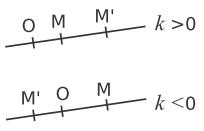
\includegraphics[scale=0.8]{img/homo_v2}	
\end{center}

\end{multicols}

\end{mydef}

\begin{myrem}
	\begin{itemize}
		\item Si $k>1$ ou $k<-1$, la figure est un agrandissement de la figure initiale.
		\item Si $-1<k<0$ ou $0<k<1$, la figure est une réduction de a figure initiale. 
	\end{itemize}
\end{myrem}

\begin{myprops}
	Par une \homo\ de rapport $k$, l'image :
	\begin{itemize}
		\item d'une droite est une droite qui lui est parallèle;
		\item d'un segment $[MN]$ est un segment $[M'N']$ de longueur $k \times MN$ (si $k>0$) ou $-k \times MN$ (si $k<0$)
	\end{itemize}
\end{myprops}

\section{Théorème de Thalès}

\begin{myact}{2 page 157}
	Le triangle AMN est l'image du triangle ABC par une \homo de rapport $k$.
	\begin{enumerate}[label=\alph*.]
		\item Le point $A$ est le centre de cette \homo .
		\item \begin{itemize}
			\item Le coté \seg{AM} est l'image de \seg{AB} par cette \homo , donc $\frac{AM}{AB}=k$.  
			\item Le coté \seg{AN} est l'image de \seg{AC} par cette \homo , donc $\frac{AN}{AC}=k$.
			\item Le coté \seg{MN} est l'image de \seg{BC} par cette \homo , donc $\frac{MN}{BC}=k$.
		\end{itemize}
		
		On a donc : \begin{equation*}
			k=\dfrac{AM}{AB}=\dfrac{AN}{AC}=\dfrac{MN}{BC}
		\end{equation*}
		
		\item La figure d'origine et l'image sont du même coté du centre de l'\homo\ $A$, donc $k$ est positif ; le triangle AMN est une réduction du triangle ABC donc $k$ est inférieur à 1. On a ici $0<k<1$. 
	\end{enumerate}
\end{myact}

\begin{myprop}
	Si deux droites \dte{BM} et \dte{CN} sécantes en $A$ sont coupées par deux droites parallèles \dte{BC} et \dte{MN}, \textbf{alors :}
		
	\begin{equation*}
		\dfrac{A\textcolor{Blue}{M}}{A\textcolor{Red}{B}}=\dfrac{A\textcolor{Blue}{N}}{A\textcolor{Red}{C}}=\dfrac{\textcolor{Blue}{MN}}{\textcolor{Red}{BC}}
	\end{equation*}
	
	\vspace*{0.5cm}
	\textbf{Configurations de Thalès :}
	\begin{multicols}{3}
		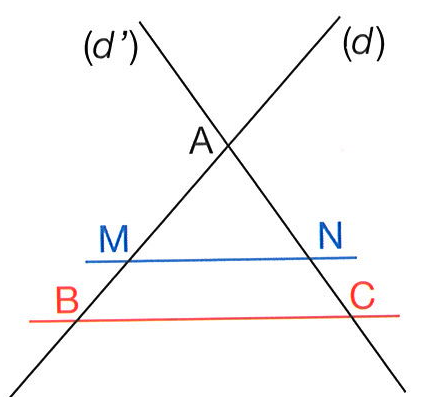
\includegraphics[scale=0.4]{./img/thales3}
		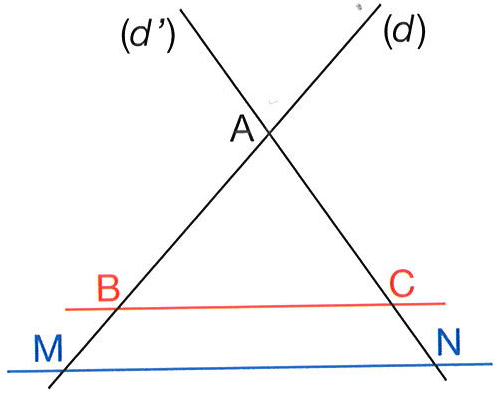
\includegraphics[scale=0.4]{./img/thales2}
		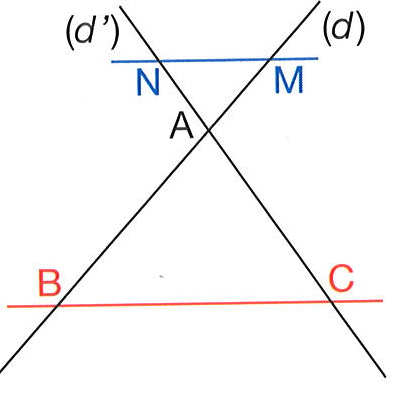
\includegraphics[scale=0.4]{./img/thales1}
	\end{multicols}
	
	Le triangle AMN est l'image du triangle ABC par une \homo\ de centre A.
\end{myprop}
\end{document}